\documentclass[10pt  ,usenames, dvipsnames]{article}\usepackage[]{graphicx}\usepackage[]{color}
%% maxwidth is the original width if it is less than linewidth
%% otherwise use linewidth (to make sure the graphics do not exceed the margin)
\makeatletter
\def\maxwidth{ %
  \ifdim\Gin@nat@width>\linewidth
    \linewidth
  \else
    \Gin@nat@width
  \fi
}
\makeatother

\definecolor{fgcolor}{rgb}{0.345, 0.345, 0.345}
\newcommand{\hlnum}[1]{\textcolor[rgb]{0.686,0.059,0.569}{#1}}%
\newcommand{\hlstr}[1]{\textcolor[rgb]{0.192,0.494,0.8}{#1}}%
\newcommand{\hlcom}[1]{\textcolor[rgb]{0.678,0.584,0.686}{\textit{#1}}}%
\newcommand{\hlopt}[1]{\textcolor[rgb]{0,0,0}{#1}}%
\newcommand{\hlstd}[1]{\textcolor[rgb]{0.345,0.345,0.345}{#1}}%
\newcommand{\hlkwa}[1]{\textcolor[rgb]{0.161,0.373,0.58}{\textbf{#1}}}%
\newcommand{\hlkwb}[1]{\textcolor[rgb]{0.69,0.353,0.396}{#1}}%
\newcommand{\hlkwc}[1]{\textcolor[rgb]{0.333,0.667,0.333}{#1}}%
\newcommand{\hlkwd}[1]{\textcolor[rgb]{0.737,0.353,0.396}{\textbf{#1}}}%
\let\hlipl\hlkwb

\usepackage{framed}
\makeatletter
\newenvironment{kframe}{%
 \def\at@end@of@kframe{}%
 \ifinner\ifhmode%
  \def\at@end@of@kframe{\end{minipage}}%
  \begin{minipage}{\columnwidth}%
 \fi\fi%
 \def\FrameCommand##1{\hskip\@totalleftmargin \hskip-\fboxsep
 \colorbox{shadecolor}{##1}\hskip-\fboxsep
     % There is no \\@totalrightmargin, so:
     \hskip-\linewidth \hskip-\@totalleftmargin \hskip\columnwidth}%
 \MakeFramed {\advance\hsize-\width
   \@totalleftmargin\z@ \linewidth\hsize
   \@setminipage}}%
 {\par\unskip\endMakeFramed%
 \at@end@of@kframe}
\makeatother

\definecolor{shadecolor}{rgb}{.97, .97, .97}
\definecolor{messagecolor}{rgb}{0, 0, 0}
\definecolor{warningcolor}{rgb}{1, 0, 1}
\definecolor{errorcolor}{rgb}{1, 0, 0}
\newenvironment{knitrout}{}{} % an empty environment to be redefined in TeX

\usepackage{alltt}
\usepackage{graphicx, verbatim}
\usepackage{amsmath}
\usepackage{amssymb}
\usepackage{amscd}
\usepackage{lipsum}
\usepackage{todonotes}
\usepackage[tableposition=top]{caption}
\usepackage{ifthen}
\usepackage[utf8]{inputenc}
\usepackage{graphicx}
\usepackage{caption}
\usepackage{listings}
\usepackage{color}
\setlength{\textwidth}{6.5in} 
\setlength{\textheight}{9in}
\setlength{\oddsidemargin}{0in} 
\setlength{\evensidemargin}{0in}
\setlength{\topmargin}{-1.5cm}
\setlength{\parindent}{0cm}
\usepackage{setspace}
\usepackage{float}
\usepackage{amssymb}
\usepackage[utf8]{inputenc}
\usepackage{fancyhdr}
\usepackage{tabularx}
\usepackage{lmodern} % for bold teletype font
\usepackage{minted}
\usepackage{underscore}

\usepackage{hyperref}
\hypersetup{
  colorlinks   = true, %Colours links instead of ugly boxes
  urlcolor     = blue, %Colour for external hyperlinks
  linkcolor    = blue, %Colour of internal links
  citecolor   = red %Colour of citations
}

%\fancyhf{}
\rfoot{Andrew Tait \thepage}
\singlespacing
\usepackage[affil-it]{authblk} 
\usepackage{etoolbox}
\usepackage{lmodern}

% Notice the following package, it will help you cite papers
\usepackage[backend=bibtex ,sorting=none]{biblatex}
\bibliography{references}
\IfFileExists{upquote.sty}{\usepackage{upquote}}{}
\begin{document}


\title{\LARGE Coursework  \\ Data Science Development (CMM535)}

\author{Andrew Tait, \textit{\href{1504693@rgu.ac.uk}{1504693@rgu.ac.uk}}}
\maketitle
% \begin{flushleft} \today \end{flushleft} 
\noindent\rule{16cm}{0.4pt}
%\underline{\hspace{3cm}
\ \\
%\thispagestyle{empty}



\section {Data Exploration}



\subsection{Dataset Choice}
The dataset that has been chosen for this part of the coursework is Mushroom. This is available on the UCI repository. The set was chosen because of it's adequate instance size and number of attributes.

\url{http://archive.ics.uci.edu/ml/datasets/Mushroom}



\subsection{Problem Statement and Data Exploration}


The main purpose of the Mushroom dataset is to identify which characteristics (attributes) determine if a particular mushroom species is editable or poisonous.

Therefore the aim of this assignment is to build a predictive model to predict if a certain type of Mushroom is ediable or not.


To start off the data explortation I will first import the required packages.

\begin{knitrout}
\definecolor{shadecolor}{rgb}{0.969, 0.969, 0.969}\color{fgcolor}\begin{kframe}
\begin{alltt}
\hlcom{#Import packages}
\hlkwd{library}\hlstd{(randomForest)}
\hlkwd{library}\hlstd{(e1071)}
\hlkwd{library}\hlstd{(caret)}
\hlkwd{library}\hlstd{(ggplot2)}
\hlkwd{library}\hlstd{(gridExtra)}
\hlkwd{library}\hlstd{(caret)}
\hlkwd{library}\hlstd{(rpart.plot)}
\hlkwd{library}\hlstd{(RColorBrewer)}
\hlkwd{library}\hlstd{(plyr)}
\hlkwd{library}\hlstd{(dplyr)}
\hlkwd{library}\hlstd{(doParallel)}
\hlkwd{library}\hlstd{(xtable)}
\end{alltt}
\end{kframe}
\end{knitrout}




Then set the working directory to the Coursework project folder path:
\begin{knitrout}
\definecolor{shadecolor}{rgb}{0.969, 0.969, 0.969}\color{fgcolor}\begin{kframe}
\begin{alltt}
\hlkwd{setwd}\hlstd{(}\hlstr{"~/CMM535 Data Science Development/Coursework/CMM535_Coursework"}\hlstd{)}
\end{alltt}
\end{kframe}
\end{knitrout}



In order to import the dataset, I used a third party helper function, which can be viewed at (Figure~\ref{figHelper})  .
The helper function not only set the attributes names but the instances names as well. Since all the data is represented a single character, it converts them into their string equivalent.


\begin{knitrout}
\definecolor{shadecolor}{rgb}{0.969, 0.969, 0.969}\color{fgcolor}\begin{kframe}
\begin{alltt}
\hlcom{#helper function}
\hlkwd{source}\hlstd{(}\hlstr{'helper_functions.r'}\hlstd{)}

\hlcom{#Import datasets using helper function}

\hlstd{mushroom} \hlkwb{<-} \hlkwd{fetchAndCleanData}\hlstd{()}
\end{alltt}
\end{kframe}
\end{knitrout}





Now that the dataset is imported, it is time to do some data exploration and analysis.

Number of rows in the dataset:

\begin{knitrout}
\definecolor{shadecolor}{rgb}{0.969, 0.969, 0.969}\color{fgcolor}\begin{kframe}
\begin{alltt}
\hlcom{#Number of rows in the dataset}
\hlkwd{nrow}\hlstd{(mushroom)}
\end{alltt}
\end{kframe}
\end{knitrout}


\begin{knitrout}
\definecolor{shadecolor}{rgb}{0.969, 0.969, 0.969}\color{fgcolor}\begin{kframe}
\begin{verbatim}
## [1] 8124
\end{verbatim}
\end{kframe}
\end{knitrout}

Number of columns (features) in the dataset:

\begin{knitrout}
\definecolor{shadecolor}{rgb}{0.969, 0.969, 0.969}\color{fgcolor}\begin{kframe}
\begin{alltt}
\hlkwd{ncol}\hlstd{(mushroom)}
\end{alltt}
\end{kframe}
\end{knitrout}


\begin{knitrout}
\definecolor{shadecolor}{rgb}{0.969, 0.969, 0.969}\color{fgcolor}\begin{kframe}
\begin{verbatim}
## [1] 23
\end{verbatim}
\end{kframe}
\end{knitrout}

Summary of the Mushroom dataset:

\begin{knitrout}
\definecolor{shadecolor}{rgb}{0.969, 0.969, 0.969}\color{fgcolor}\begin{kframe}
\begin{alltt}
\hlcom{#Summary of the Mushroom dataset}
\hlkwd{str}\hlstd{(mushroom)}
\end{alltt}
\end{kframe}
\end{knitrout}


\begin{knitrout}
\definecolor{shadecolor}{rgb}{0.969, 0.969, 0.969}\color{fgcolor}\begin{kframe}
\begin{verbatim}
## 'data.frame':	8124 obs. of  23 variables:
##  $ Edible               : Factor w/ 2 levels "Edible","Poisonous": 2 1 1 2 1 1 1 1 2 1 ...
##  $ CapShape             : Factor w/ 12 levels "b","c","f","k",..: 9 9 7 9 9 9 7 7 9 7 ...
##  $ CapSurface           : Factor w/ 8 levels "f","g","s","y",..: 8 8 8 7 8 7 8 7 7 8 ...
##  $ CapColor             : Factor w/ 20 levels "b","c","e","g",..: 11 20 19 19 14 20 19 19 19 20 ...
##  $ Bruises              : Factor w/ 4 levels "f","t","True",..: 3 3 3 3 4 3 3 3 3 3 ...
##  $ Odor                 : Factor w/ 18 levels "a","c","f","l",..: 17 10 11 17 16 10 10 11 17 10 ...
##  $ GillAttachment       : Factor w/ 6 levels "a","f","Attached",..: 5 5 5 5 5 5 5 5 5 5 ...
##  $ GillSpacing          : Factor w/ 5 levels "c","w","Close",..: 3 3 3 3 4 3 3 3 3 3 ...
##  $ GillSize             : Factor w/ 4 levels "b","n","Broad",..: 4 3 3 4 3 3 3 3 4 3 ...
##  $ GillColor            : Factor w/ 24 levels "b","e","g","h",..: 13 13 14 14 13 14 17 14 20 17 ...
##  $ StalkShape           : Factor w/ 4 levels "e","t","Enlarging",..: 3 3 3 3 4 3 3 3 3 3 ...
##  $ StalkRoot            : Factor w/ 12 levels "?","b","c","e",..: 9 7 7 9 9 7 7 7 9 7 ...
##  $ StalkSurfaceAboveRing: Factor w/ 8 levels "f","k","s","y",..: 8 8 8 8 8 8 8 8 8 8 ...
##  $ StalkSurfaceBelowRing: Factor w/ 8 levels "f","k","s","y",..: 8 8 8 8 8 8 8 8 8 8 ...
##  $ StalkColorAboveRing  : Factor w/ 18 levels "b","c","e","g",..: 17 17 17 17 17 17 17 17 17 17 ...
##  $ StalkColorBelowRing  : Factor w/ 18 levels "b","c","e","g",..: 17 17 17 17 17 17 17 17 17 17 ...
##  $ VeilType             : Factor w/ 3 levels "p","Partial",..: 2 2 2 2 2 2 2 2 2 2 ...
##  $ VeilColor            : Factor w/ 8 levels "n","o","w","y",..: 7 7 7 7 7 7 7 7 7 7 ...
##  $ RingNumber           : Factor w/ 6 levels "n","o","t","None",..: 5 5 5 5 5 5 5 5 5 5 ...
##  $ RingType             : Factor w/ 13 levels "e","f","l","n",..: 11 11 11 11 7 11 11 11 11 11 ...
##  $ SporePrintColor      : Factor w/ 18 levels "b","h","k","n",..: 10 11 11 10 11 10 10 11 10 10 ...
##  $ Population           : Factor w/ 12 levels "a","c","n","s",..: 10 9 9 10 7 9 9 10 11 10 ...
##  $ Habitat              : Factor w/ 14 levels "d","g","l","m",..: 12 8 10 12 8 8 10 10 8 10 ...
\end{verbatim}
\end{kframe}
\end{knitrout}

Now that some basic data exploration is covered, next to inspect the dataset a bit further. Starting with the class (Edible) distribution in the mushroom dataset, see (Figure~\ref{fig1})

\begin{knitrout}
\definecolor{shadecolor}{rgb}{0.969, 0.969, 0.969}\color{fgcolor}\begin{kframe}
\begin{alltt}
\hlcom{#Class Distribution}
\hlkwd{barplot}\hlstd{(}\hlkwd{table}\hlstd{(mushroom}\hlopt{$}\hlstd{Edible))}
\end{alltt}
\end{kframe}
\end{knitrout}
\begin{figure}[H]
\begin{center}
\begin{knitrout}
\definecolor{shadecolor}{rgb}{0.969, 0.969, 0.969}\color{fgcolor}
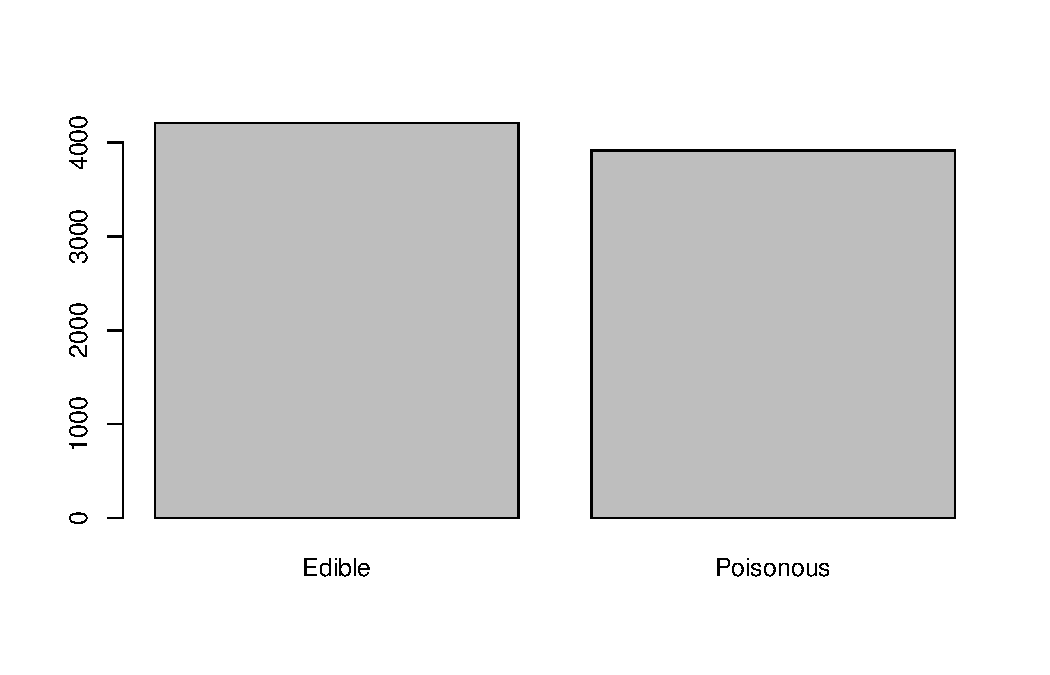
\includegraphics[width=.76\linewidth]{figure/unnamed-chunk-14-1} 

\end{knitrout}
\caption {Barplot of Class Distribution}
\label{fig1}
\end {center}
\end {figure}

Next is to analyse if there is a correlocation between the CapShape and CapSurface of a mushroom and whether it is Edible or Poisonous. Which is shown in the plot ((Figure~\ref{fig2})) below.

\begin{knitrout}
\definecolor{shadecolor}{rgb}{0.969, 0.969, 0.969}\color{fgcolor}\begin{kframe}
\begin{alltt}
\hlcom{#Comparisons of CapShape and CapSurface with Edible or Poisonous}
\hlkwd{ggplot}\hlstd{(mushroom,}\hlkwd{aes}\hlstd{(}\hlkwc{x}\hlstd{=CapShape,} \hlkwc{y}\hlstd{=CapSurface,} \hlkwc{color}\hlstd{=Edible))} \hlopt{+}
                       \hlkwd{geom_jitter}\hlstd{(}\hlkwc{alpha}\hlstd{=}\hlnum{0.3}\hlstd{)} \hlopt{+}
                       \hlkwd{scale_color_manual}\hlstd{(}\hlkwc{breaks} \hlstd{=} \hlkwd{c}\hlstd{(}\hlstr{'Edible'}\hlstd{,}\hlstr{'Poisonous'}\hlstd{),}
                                          \hlkwc{values}\hlstd{=}\hlkwd{c}\hlstd{(}\hlstr{'darkgreen'}\hlstd{,}\hlstr{'red'}\hlstd{))}
\end{alltt}
\end{kframe}
\end{knitrout}

\begin{figure}[H]
\begin{center}
\begin{knitrout}
\definecolor{shadecolor}{rgb}{0.969, 0.969, 0.969}\color{fgcolor}
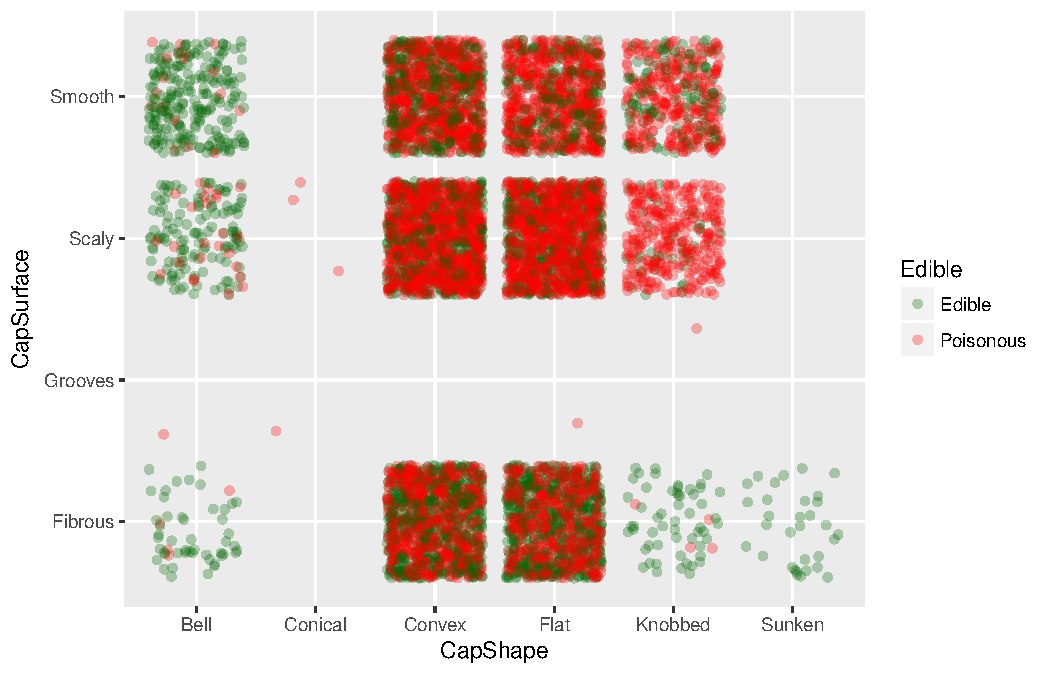
\includegraphics[width=.76\linewidth]{figure/unnamed-chunk-16-1} 

\end{knitrout}
\caption {Comparisons of CapShape and CapSurface with Edible or Poisonous in Mushroom Dataset}
\label{fig2}
\end {center}
\end {figure}

\begin{knitrout}
\definecolor{shadecolor}{rgb}{0.969, 0.969, 0.969}\color{fgcolor}\begin{kframe}
\begin{alltt}
\hlcom{#Comparisons of StalkSurfaceAboveRing and StalkSurfaceBelowRing with Edible or Poisionous}
\hlkwd{ggplot}\hlstd{(mushroom,}\hlkwd{aes}\hlstd{(}\hlkwc{x}\hlstd{=StalkSurfaceAboveRing,} \hlkwc{y}\hlstd{=StalkSurfaceBelowRing,} \hlkwc{color}\hlstd{=Edible))} \hlopt{+}
  \hlkwd{geom_jitter}\hlstd{(}\hlkwc{alpha}\hlstd{=}\hlnum{0.3}\hlstd{)} \hlopt{+}
  \hlkwd{scale_color_manual}\hlstd{(}\hlkwc{breaks} \hlstd{=} \hlkwd{c}\hlstd{(}\hlstr{'Edible'}\hlstd{,}\hlstr{'Poisonous'}\hlstd{),} \hlkwc{values}\hlstd{=}\hlkwd{c}\hlstd{(}\hlstr{'darkgreen'}\hlstd{,}\hlstr{'red'}\hlstd{))}
\end{alltt}
\end{kframe}
\end{knitrout}

\begin{figure}[H]
\begin{center}
\begin{knitrout}
\definecolor{shadecolor}{rgb}{0.969, 0.969, 0.969}\color{fgcolor}
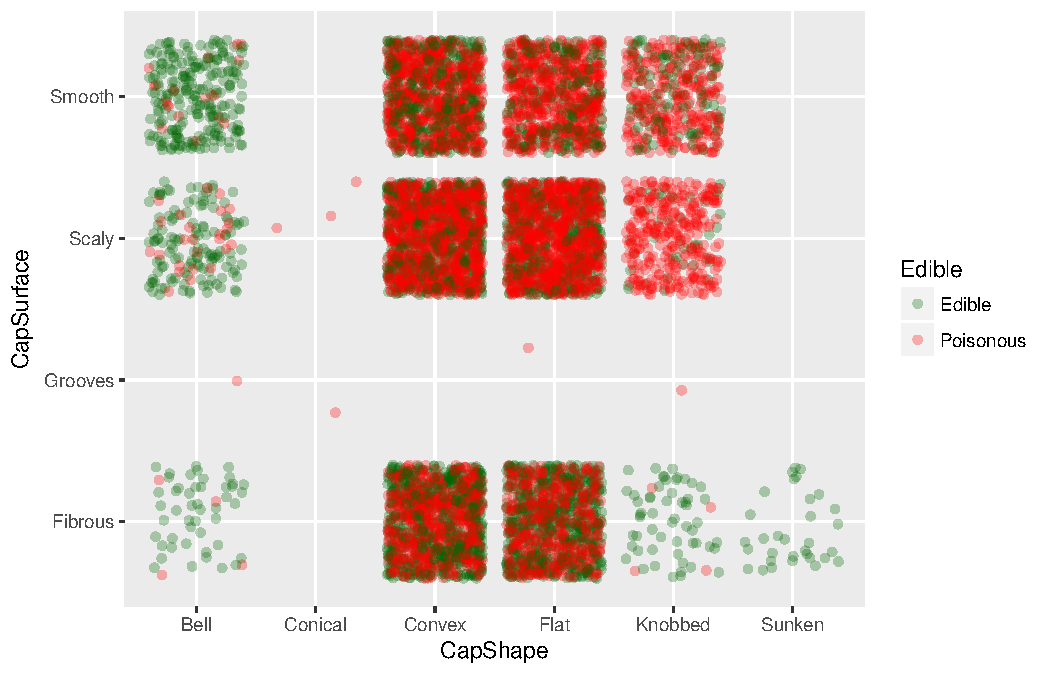
\includegraphics[width=.76\linewidth]{figure/unnamed-chunk-18-1} 

\end{knitrout}
\caption {Comparisons of StalkSurfaceAboveRing and StalkSurfaceBelowRing with Edible or Poisionous}
\label{fig3}
\end {center}
\end {figure}



\clearpage

\subsection {Pre-Processing}

Before the Mushroom dataset can be processed by a classification model(s), some pre-processing is required.

While the helper function should take out all missing values, lets valdiate this before continuing.

\begin{knitrout}
\definecolor{shadecolor}{rgb}{0.969, 0.969, 0.969}\color{fgcolor}\begin{kframe}
\begin{alltt}
\hlcom{#Class Distribution}
\hlkwd{table}\hlstd{(}\hlkwd{complete.cases} \hlstd{(mushroom))}
\end{alltt}
\end{kframe}
\end{knitrout}


\begin{knitrout}
\definecolor{shadecolor}{rgb}{0.969, 0.969, 0.969}\color{fgcolor}\begin{kframe}
\begin{verbatim}
## 
## TRUE 
## 8124
\end{verbatim}
\end{kframe}
\end{knitrout}

As shown above, there is not any missing values in the dataset.


\clearpage



\section {Modeling and Classifcation}



\subsection {Divide into training and testing subset}

When it came to dividing the mushroom dataset into training and testing subsets, I decided to go with the conventional 70 percent
training and 30 percent testing split as a starting point/baseline.

\begin{knitrout}
\definecolor{shadecolor}{rgb}{0.969, 0.969, 0.969}\color{fgcolor}\begin{kframe}
\begin{alltt}
\hlcom{#Divide the datset into 70% training and 30% testing.}
\hlstd{inTrain} \hlkwb{<-} \hlkwd{createDataPartition}\hlstd{(}\hlkwc{y}\hlstd{=mushroom}\hlopt{$}\hlstd{Edible,} \hlkwc{p}\hlstd{=}\hlnum{0.7}\hlstd{,} \hlkwc{list}\hlstd{=}\hlnum{FALSE}\hlstd{)}

\hlcom{#Assign indexes to split the Mushroom dataset into training and testing}
\hlstd{training} \hlkwb{<-} \hlstd{mushroom[inTrain,]}
\hlstd{testing} \hlkwb{<-} \hlstd{mushroom[}\hlopt{-}\hlstd{inTrain,]}
\end{alltt}
\end{kframe}
\end{knitrout}





\subsection{Build Classifier}

For the initial classifier I decided to go with the kNN Classifer as it has proven to be a good baseline in previous labs and exercises in R.



Before the classification begins, parallel processing is enabled to speed up this process.

\begin{knitrout}
\definecolor{shadecolor}{rgb}{0.969, 0.969, 0.969}\color{fgcolor}\begin{kframe}
\begin{alltt}
\hlcom{#Setup Parallel processing to speed up classification modelling }
\hlstd{cl} \hlkwb{<-} \hlkwd{makeCluster}\hlstd{(}\hlkwd{detectCores}\hlstd{(),} \hlkwc{type}\hlstd{=}\hlstr{'PSOCK'}\hlstd{)}
\hlkwd{registerDoParallel}\hlstd{(cl)}
\end{alltt}
\end{kframe}
\end{knitrout}



The train control is set to cross-validation with 5 folds:
\begin{knitrout}
\definecolor{shadecolor}{rgb}{0.969, 0.969, 0.969}\color{fgcolor}\begin{kframe}
\begin{alltt}
\hlcom{#set train control to cross-validation with 5 folds}
\hlstd{train_control}\hlkwb{<-} \hlkwd{trainControl}\hlstd{(}\hlkwc{method}\hlstd{=}\hlstr{"cv"}\hlstd{,} \hlkwc{number}\hlstd{=}\hlnum{5}\hlstd{)}
\end{alltt}
\end{kframe}
\end{knitrout}



% 
% Next the seed is set to 1, in order to make the module reproducible and the kNN model is set up with the train_control from above and the tunelength of 20.
\begin{knitrout}
\definecolor{shadecolor}{rgb}{0.969, 0.969, 0.969}\color{fgcolor}\begin{kframe}
\begin{alltt}
\hlcom{#First set the seed for reproducibility}
\hlkwd{set.seed}\hlstd{(}\hlnum{1}\hlstd{)}

\hlcom{#train model using kNN}
\hlstd{kNNModel} \hlkwb{<-} \hlkwd{train}\hlstd{(Edible} \hlopt{~} \hlstd{.,} \hlkwc{data} \hlstd{= training,}
                  \hlkwc{trControl} \hlstd{= train_control,}
                  \hlkwc{tuneLength} \hlstd{=} \hlnum{20}\hlstd{,}
                  \hlkwc{method} \hlstd{=} \hlstr{"knn"}
\hlstd{)}
\end{alltt}
\end{kframe}
\end{knitrout}




Once the knn Model is complete, it's time to analyse the results, first with a print of the kNNModel as shown below.

\begin{knitrout}
\definecolor{shadecolor}{rgb}{0.969, 0.969, 0.969}\color{fgcolor}\begin{kframe}
\begin{alltt}
\hlcom{#Show the kNN model results}
\hlstd{kNNModel}
\end{alltt}
\end{kframe}
\end{knitrout}



\begin{knitrout}
\definecolor{shadecolor}{rgb}{0.969, 0.969, 0.969}\color{fgcolor}\begin{kframe}
\begin{verbatim}
## k-Nearest Neighbors 
## 
## 5688 samples
##   22 predictor
##    2 classes: 'Edible', 'Poisonous' 
## 
## No pre-processing
## Resampling: Cross-Validated (5 fold) 
## Summary of sample sizes: 4551, 4549, 4551, 4551, 4550 
## Resampling results across tuning parameters:
## 
##   k   Accuracy   Kappa    
##    5  0.9992964  0.9985907
##    7  0.9989446  0.9978860
##    9  0.9987687  0.9975336
##   11  0.9984169  0.9968289
##   13  0.9980654  0.9961249
##   15  0.9978895  0.9957725
##   17  0.9980654  0.9961249
##   19  0.9975377  0.9950681
##   21  0.9973618  0.9947159
##   23  0.9975377  0.9950683
##   25  0.9971863  0.9943648
##   27  0.9966591  0.9933090
##   29  0.9959561  0.9919015
##   31  0.9954287  0.9908461
##   33  0.9950768  0.9901412
##   35  0.9945492  0.9890853
##   37  0.9940215  0.9880294
##   39  0.9933181  0.9866213
##   41  0.9920878  0.9841591
##   43  0.9908568  0.9816959
## 
## Accuracy was used to select the optimal model using the largest value.
## The final value used for the model was k = 5.
\end{verbatim}
\end{kframe}
\end{knitrout}


Next is a confusion matrix is created by predicting the accuracy against the testing subset.

\begin{knitrout}
\definecolor{shadecolor}{rgb}{0.969, 0.969, 0.969}\color{fgcolor}\begin{kframe}
\begin{alltt}
\hlcom{#Predict the accuracy of the kNN Model against the testing set}
\hlstd{predictkNN} \hlkwb{<-} \hlkwd{predict}\hlstd{(kNNModel,testing)}
\hlkwd{confusionMatrix}\hlstd{(predictkNN, testing}\hlopt{$}\hlstd{Edible)}
\end{alltt}
\end{kframe}
\end{knitrout}



\begin{knitrout}
\definecolor{shadecolor}{rgb}{0.969, 0.969, 0.969}\color{fgcolor}\begin{kframe}
\begin{verbatim}
## Confusion Matrix and Statistics
## 
##            Reference
## Prediction  Edible Poisonous
##   Edible      1262         0
##   Poisonous      0      1174
##                                      
##                Accuracy : 1          
##                  95% CI : (0.9985, 1)
##     No Information Rate : 0.5181     
##     P-Value [Acc > NIR] : < 2.2e-16  
##                                      
##                   Kappa : 1          
##  Mcnemar's Test P-Value : NA         
##                                      
##             Sensitivity : 1.0000     
##             Specificity : 1.0000     
##          Pos Pred Value : 1.0000     
##          Neg Pred Value : 1.0000     
##              Prevalence : 0.5181     
##          Detection Rate : 0.5181     
##    Detection Prevalence : 0.5181     
##       Balanced Accuracy : 1.0000     
##                                      
##        'Positive' Class : Edible     
## 
\end{verbatim}
\end{kframe}
\end{knitrout}




\clearpage


\subsection{Improve Model Performance}

\subsubsection{C5.0 Model}

\begin{knitrout}
\definecolor{shadecolor}{rgb}{0.969, 0.969, 0.969}\color{fgcolor}\begin{kframe}
\begin{alltt}
\hlcom{#First set the seed for reproducibility}
\hlkwd{set.seed}\hlstd{(}\hlnum{1}\hlstd{)}

\hlcom{#train the model using c5.0}
\hlstd{c50Model}\hlkwb{<-} \hlkwd{train}\hlstd{(Edible}\hlopt{~}\hlstd{.,} \hlkwc{data}\hlstd{=training,}
                 \hlkwc{trControl}\hlstd{=train_control,}
                 \hlkwc{tuneLength}\hlstd{=}\hlnum{5}\hlstd{,}
                 \hlkwc{method}\hlstd{=}\hlstr{"C5.0"}
\hlstd{)}
\end{alltt}
\end{kframe}
\end{knitrout}





\begin{knitrout}
\definecolor{shadecolor}{rgb}{0.969, 0.969, 0.969}\color{fgcolor}\begin{kframe}
\begin{alltt}
\hlcom{#Show the c50Model results}
 \hlstd{c50Model}
\end{alltt}
\end{kframe}
\end{knitrout}




\begin{knitrout}
\definecolor{shadecolor}{rgb}{0.969, 0.969, 0.969}\color{fgcolor}\begin{kframe}
\begin{verbatim}
## C5.0 
## 
## 5688 samples
##   22 predictor
##    2 classes: 'Edible', 'Poisonous' 
## 
## No pre-processing
## Resampling: Cross-Validated (5 fold) 
## Summary of sample sizes: 4551, 4549, 4551, 4551, 4550 
## Resampling results across tuning parameters:
## 
##   model  winnow  trials  Accuracy   Kappa    
##   rules  FALSE    1      1.0000000  1.0000000
##   rules  FALSE   10      1.0000000  1.0000000
##   rules  FALSE   20      1.0000000  1.0000000
##   rules  FALSE   30      1.0000000  1.0000000
##   rules  FALSE   40      1.0000000  1.0000000
##   rules  FALSE   50      1.0000000  1.0000000
##   rules  FALSE   60      1.0000000  1.0000000
##   rules  FALSE   70      1.0000000  1.0000000
##   rules  FALSE   80      1.0000000  1.0000000
##   rules  FALSE   90      1.0000000  1.0000000
##   rules   TRUE    1      0.9991216  0.9982406
##   rules   TRUE   10      1.0000000  1.0000000
##   rules   TRUE   20      1.0000000  1.0000000
##   rules   TRUE   30      1.0000000  1.0000000
##   rules   TRUE   40      0.9996485  0.9992961
##   rules   TRUE   50      0.9996485  0.9992961
##   rules   TRUE   60      0.9996485  0.9992961
##   rules   TRUE   70      0.9996485  0.9992961
##   rules   TRUE   80      0.9996485  0.9992961
##   rules   TRUE   90      0.9996485  0.9992961
##   tree   FALSE    1      1.0000000  1.0000000
##   tree   FALSE   10      1.0000000  1.0000000
##   tree   FALSE   20      1.0000000  1.0000000
##   tree   FALSE   30      1.0000000  1.0000000
##   tree   FALSE   40      1.0000000  1.0000000
##   tree   FALSE   50      1.0000000  1.0000000
##   tree   FALSE   60      1.0000000  1.0000000
##   tree   FALSE   70      1.0000000  1.0000000
##   tree   FALSE   80      1.0000000  1.0000000
##   tree   FALSE   90      1.0000000  1.0000000
##   tree    TRUE    1      0.9994728  0.9989440
##   tree    TRUE   10      1.0000000  1.0000000
##   tree    TRUE   20      1.0000000  1.0000000
##   tree    TRUE   30      1.0000000  1.0000000
##   tree    TRUE   40      1.0000000  1.0000000
##   tree    TRUE   50      1.0000000  1.0000000
##   tree    TRUE   60      1.0000000  1.0000000
##   tree    TRUE   70      1.0000000  1.0000000
##   tree    TRUE   80      1.0000000  1.0000000
##   tree    TRUE   90      1.0000000  1.0000000
## 
## Accuracy was used to select the optimal model using the largest value.
## The final values used for the model were trials = 1, model = rules
##  and winnow = FALSE.
\end{verbatim}
\end{kframe}
\end{knitrout}



\begin{knitrout}
\definecolor{shadecolor}{rgb}{0.969, 0.969, 0.969}\color{fgcolor}\begin{kframe}
\begin{alltt}
\hlstd{predictC50} \hlkwb{<-} \hlkwd{predict}\hlstd{(c50Model, testing)}
\hlkwd{confusionMatrix}\hlstd{(predictC50,testing}\hlopt{$}\hlstd{Edible)}
\end{alltt}
\end{kframe}
\end{knitrout}




\begin{knitrout}
\definecolor{shadecolor}{rgb}{0.969, 0.969, 0.969}\color{fgcolor}\begin{kframe}
\begin{verbatim}
## Confusion Matrix and Statistics
## 
##            Reference
## Prediction  Edible Poisonous
##   Edible      1262         0
##   Poisonous      0      1174
##                                      
##                Accuracy : 1          
##                  95% CI : (0.9985, 1)
##     No Information Rate : 0.5181     
##     P-Value [Acc > NIR] : < 2.2e-16  
##                                      
##                   Kappa : 1          
##  Mcnemar's Test P-Value : NA         
##                                      
##             Sensitivity : 1.0000     
##             Specificity : 1.0000     
##          Pos Pred Value : 1.0000     
##          Neg Pred Value : 1.0000     
##              Prevalence : 0.5181     
##          Detection Rate : 0.5181     
##    Detection Prevalence : 0.5181     
##       Balanced Accuracy : 1.0000     
##                                      
##        'Positive' Class : Edible     
## 
\end{verbatim}
\end{kframe}
\end{knitrout}




\clearpage

\subsubsection{Random forest Model}

\begin{knitrout}
\definecolor{shadecolor}{rgb}{0.969, 0.969, 0.969}\color{fgcolor}\begin{kframe}
\begin{alltt}
\hlcom{#First set the seed for reproducibility}
\hlkwd{set.seed}\hlstd{(}\hlnum{1}\hlstd{)}

\hlcom{# train the model using random forest}
\hlstd{RFModel}\hlkwb{<-} \hlkwd{train}\hlstd{(Edible}\hlopt{~}\hlstd{.,} \hlkwc{data}\hlstd{=training,}
                \hlkwc{trControl}\hlstd{=train_control,}
                \hlkwc{method}\hlstd{=}\hlstr{"rf"}\hlstd{,}
                \hlkwc{tuneLength} \hlstd{=}\hlnum{10}\hlstd{,}
                \hlkwc{metric} \hlstd{=} \hlstr{'Accuracy'}
\hlstd{)}
\end{alltt}
\end{kframe}
\end{knitrout}




\begin{knitrout}
\definecolor{shadecolor}{rgb}{0.969, 0.969, 0.969}\color{fgcolor}\begin{kframe}
\begin{alltt}
\hlstd{RFModel}
\end{alltt}
\end{kframe}
\end{knitrout}


\begin{knitrout}
\definecolor{shadecolor}{rgb}{0.969, 0.969, 0.969}\color{fgcolor}\begin{kframe}
\begin{verbatim}
## Random Forest 
## 
## 5688 samples
##   22 predictor
##    2 classes: 'Edible', 'Poisonous' 
## 
## No pre-processing
## Resampling: Cross-Validated (5 fold) 
## Summary of sample sizes: 4551, 4549, 4551, 4551, 4550 
## Resampling results across tuning parameters:
## 
##   mtry  Accuracy   Kappa    
##     2   0.8957470  0.7896431
##    26   1.0000000  1.0000000
##    50   1.0000000  1.0000000
##    75   1.0000000  1.0000000
##    99   1.0000000  1.0000000
##   123   0.9998241  0.9996477
##   148   0.9998241  0.9996477
##   172   0.9996484  0.9992958
##   196   0.9996484  0.9992958
##   221   0.9996484  0.9992958
## 
## Accuracy was used to select the optimal model using the largest value.
## The final value used for the model was mtry = 26.
\end{verbatim}
\end{kframe}
\end{knitrout}

\begin{knitrout}
\definecolor{shadecolor}{rgb}{0.969, 0.969, 0.969}\color{fgcolor}\begin{kframe}
\begin{alltt}
\hlstd{predictRF} \hlkwb{<-} \hlkwd{predict}\hlstd{(RFModel,testing)}
\hlkwd{confusionMatrix}\hlstd{(predictRF, testing}\hlopt{$}\hlstd{Edible)}
\end{alltt}
\end{kframe}
\end{knitrout}


\begin{knitrout}
\definecolor{shadecolor}{rgb}{0.969, 0.969, 0.969}\color{fgcolor}\begin{kframe}
\begin{verbatim}
## Confusion Matrix and Statistics
## 
##            Reference
## Prediction  Edible Poisonous
##   Edible      1262         0
##   Poisonous      0      1174
##                                      
##                Accuracy : 1          
##                  95% CI : (0.9985, 1)
##     No Information Rate : 0.5181     
##     P-Value [Acc > NIR] : < 2.2e-16  
##                                      
##                   Kappa : 1          
##  Mcnemar's Test P-Value : NA         
##                                      
##             Sensitivity : 1.0000     
##             Specificity : 1.0000     
##          Pos Pred Value : 1.0000     
##          Neg Pred Value : 1.0000     
##              Prevalence : 0.5181     
##          Detection Rate : 0.5181     
##    Detection Prevalence : 0.5181     
##       Balanced Accuracy : 1.0000     
##                                      
##        'Positive' Class : Edible     
## 
\end{verbatim}
\end{kframe}
\end{knitrout}



\clearpage


\subsubsection{Comparison of all Models}




\begin{knitrout}
\definecolor{shadecolor}{rgb}{0.969, 0.969, 0.969}\color{fgcolor}\begin{kframe}
\begin{verbatim}
## Confusion Matrix and Statistics
## 
##            Reference
## Prediction  Edible Poisonous
##   Edible      1262         0
##   Poisonous      0      1174
##                                      
##                Accuracy : 1          
##                  95% CI : (0.9985, 1)
##     No Information Rate : 0.5181     
##     P-Value [Acc > NIR] : < 2.2e-16  
##                                      
##                   Kappa : 1          
##  Mcnemar's Test P-Value : NA         
##                                      
##             Sensitivity : 1.0000     
##             Specificity : 1.0000     
##          Pos Pred Value : 1.0000     
##          Neg Pred Value : 1.0000     
##              Prevalence : 0.5181     
##          Detection Rate : 0.5181     
##    Detection Prevalence : 0.5181     
##       Balanced Accuracy : 1.0000     
##                                      
##        'Positive' Class : Edible     
## 
\end{verbatim}
\end{kframe}
\end{knitrout}


\clearpage



\section{Fine-grained Model}


\subsection{Clustering Dataset}

\subsubsection{Pre-processing}

\begin{knitrout}
\definecolor{shadecolor}{rgb}{0.969, 0.969, 0.969}\color{fgcolor}\begin{kframe}
\begin{alltt}
\hlstd{normalizeData} \hlkwb{<-} \hlkwa{function} \hlstd{(}\hlkwc{x} \hlstd{) \{}
\hlkwd{return} \hlstd{( (x}\hlopt{-}\hlkwd{min}\hlstd{(x) )} \hlopt{/} \hlstd{(} \hlkwd{max}\hlstd{(x)}\hlopt{-} \hlkwd{min}\hlstd{(x) ))}
\hlstd{\}}
\end{alltt}
\end{kframe}
\end{knitrout}






% Clustering function to run (displayed as a listing at the end of the doc)



\begin{knitrout}
\definecolor{shadecolor}{rgb}{0.969, 0.969, 0.969}\color{fgcolor}\begin{kframe}
\begin{alltt}
\hlcom{#Copy the dataset before pre-processing }
\hlstd{dfNew} \hlkwb{<-} \hlstd{mushroom}
\hlstd{dfNew}\hlopt{$}\hlstd{VeilType} \hlkwb{<-} \hlkwa{NULL}

\hlcom{#Convert the dataframe to numeric values}
\hlstd{dfNew[,}\hlnum{2}\hlopt{:}\hlnum{22}\hlstd{]} \hlkwb{=} \hlkwd{lapply}\hlstd{(dfNew[,}\hlnum{2}\hlopt{:}\hlnum{22}\hlstd{], as.numeric)}

\hlcom{##Then use the normalise function from above}
\hlstd{dfN} \hlkwb{<-} \hlkwd{as.data.frame}\hlstd{(}\hlkwd{lapply}\hlstd{(dfNew[,}\hlopt{-}\hlnum{1}\hlstd{], normalizeData))}
\end{alltt}
\end{kframe}
\end{knitrout}





\subsubsection{Clustering using clustData function}

\begin{knitrout}
\definecolor{shadecolor}{rgb}{0.969, 0.969, 0.969}\color{fgcolor}\begin{kframe}
\begin{alltt}
\hlkwd{str}\hlstd{(dfN)}
\hlstd{dfN}\hlopt{$}\hlstd{Edible} \hlkwb{<-} \hlstd{dfNew}\hlopt{$}\hlstd{Edible}

\hlkwd{table}\hlstd{(}\hlkwd{complete.cases} \hlstd{(dfN))}
\end{alltt}
\end{kframe}
\end{knitrout}


\begin{knitrout}
\definecolor{shadecolor}{rgb}{0.969, 0.969, 0.969}\color{fgcolor}\begin{kframe}
\begin{verbatim}
## 'data.frame':	8124 obs. of  21 variables:
##  $ CapShape             : num  0.4 0.4 0 0.4 0.4 0.4 0 0 0.4 0 ...
##  $ CapSurface           : num  1 1 1 0.667 1 ...
##  $ CapColor             : num  0 1 0.889 0.889 0.333 ...
##  $ Bruises              : num  0 0 0 0 1 0 0 0 0 0 ...
##  $ Odor                 : num  0.875 0 0.125 0.875 0.75 0 0 0.125 0.875 0 ...
##  $ GillAttachment       : num  1 1 1 1 1 1 1 1 1 1 ...
##  $ GillSpacing          : num  0 0 0 0 1 0 0 0 0 0 ...
##  $ GillSize             : num  1 0 0 1 0 0 0 0 1 0 ...
##  $ GillColor            : num  0 0 0.0909 0.0909 0 ...
##  $ StalkShape           : num  0 0 0 0 1 0 0 0 0 0 ...
##  $ StalkRoot            : num  0.5 0.167 0.167 0.5 0.5 ...
##  $ StalkSurfaceAboveRing: num  1 1 1 1 1 1 1 1 1 1 ...
##  $ StalkSurfaceBelowRing: num  1 1 1 1 1 1 1 1 1 1 ...
##  $ StalkColorAboveRing  : num  0.875 0.875 0.875 0.875 0.875 0.875 0.875 0.875 0.875 0.875 ...
##  $ StalkColorBelowRing  : num  0.875 0.875 0.875 0.875 0.875 0.875 0.875 0.875 0.875 0.875 ...
##  $ VeilColor            : num  0.667 0.667 0.667 0.667 0.667 ...
##  $ RingNumber           : num  0.5 0.5 0.5 0.5 0.5 0.5 0.5 0.5 0.5 0.5 ...
##  $ RingType             : num  1 1 1 1 0 1 1 1 1 1 ...
##  $ SporePrintColor      : num  0 0.125 0.125 0 0.125 0 0 0.125 0 0 ...
##  $ Population           : num  0.6 0.4 0.4 0.6 0 0.4 0.4 0.6 0.8 0.6 ...
##  $ Habitat              : num  0.667 0 0.333 0.667 0 ...
## 
## TRUE 
## 8124
\end{verbatim}
\end{kframe}
\end{knitrout}

\begin{knitrout}
\definecolor{shadecolor}{rgb}{0.969, 0.969, 0.969}\color{fgcolor}\begin{kframe}
\begin{alltt}
\hlstd{clusteredDF} \hlkwb{<-} \hlkwd{clustData}\hlstd{(dfN,}\hlkwd{ncol}\hlstd{(dfNew),} \hlkwd{c}\hlstd{(}\hlnum{2}\hlstd{,}\hlnum{2}\hlstd{))}
\hlkwd{head}\hlstd{(clusteredDF,}\hlnum{10}\hlstd{)}
\end{alltt}
\end{kframe}
\end{knitrout}

\begin{knitrout}
\definecolor{shadecolor}{rgb}{0.969, 0.969, 0.969}\color{fgcolor}\begin{kframe}
\begin{verbatim}
##    CapShape CapSurface  CapColor Bruises  Odor GillAttachment GillSpacing
## 1       0.4  1.0000000 1.0000000       0 0.000              1           0
## 2       0.0  1.0000000 0.8888889       0 0.125              1           0
## 3       0.4  1.0000000 0.3333333       1 0.750              1           1
## 4       0.4  0.6666667 1.0000000       0 0.000              1           0
## 5       0.0  1.0000000 0.8888889       0 0.000              1           0
## 6       0.0  0.6666667 0.8888889       0 0.125              1           0
## 7       0.0  1.0000000 1.0000000       0 0.000              1           0
## 8       0.4  0.6666667 1.0000000       0 0.125              1           0
## 9       0.4  0.6666667 1.0000000       0 0.000              1           0
## 10      0.0  1.0000000 1.0000000       0 0.000              1           0
##    GillSize  GillColor StalkShape StalkRoot StalkSurfaceAboveRing
## 1         0 0.00000000          0 0.1666667                     1
## 2         0 0.09090909          0 0.1666667                     1
## 3         0 0.00000000          1 0.5000000                     1
## 4         0 0.09090909          0 0.1666667                     1
## 5         0 0.36363636          0 0.1666667                     1
## 6         0 0.09090909          0 0.1666667                     1
## 7         0 0.36363636          0 0.1666667                     1
## 8         0 0.36363636          0 0.1666667                     1
## 9         0 0.09090909          0 0.1666667                     1
## 10        0 0.90909091          0 0.1666667                     1
##    StalkSurfaceBelowRing StalkColorAboveRing StalkColorBelowRing VeilColor
## 1                      1               0.875               0.875 0.6666667
## 2                      1               0.875               0.875 0.6666667
## 3                      1               0.875               0.875 0.6666667
## 4                      1               0.875               0.875 0.6666667
## 5                      1               0.875               0.875 0.6666667
## 6                      1               0.875               0.875 0.6666667
## 7                      1               0.875               0.875 0.6666667
## 8                      1               0.875               0.875 0.6666667
## 9                      1               0.875               0.875 0.6666667
## 10                     1               0.875               0.875 0.6666667
##    RingNumber RingType SporePrintColor Population   Habitat   cluster
## 1         0.5        1           0.125        0.4 0.0000000 Edible_c2
## 2         0.5        1           0.125        0.4 0.3333333 Edible_c2
## 3         0.5        0           0.125        0.0 0.0000000 Edible_c2
## 4         0.5        1           0.000        0.4 0.0000000 Edible_c2
## 5         0.5        1           0.000        0.4 0.3333333 Edible_c2
## 6         0.5        1           0.125        0.6 0.3333333 Edible_c2
## 7         0.5        1           0.000        0.6 0.3333333 Edible_c2
## 8         0.5        1           0.125        0.4 0.0000000 Edible_c2
## 9         0.5        1           0.000        0.6 0.3333333 Edible_c2
## 10        0.5        1           0.125        0.6 0.0000000 Edible_c2
\end{verbatim}
\end{kframe}
\end{knitrout}

\clearpage
\subsection{Adapting your Model}


\subsubsection{Refitting Random Forest to Clustering}

\begin{knitrout}
\definecolor{shadecolor}{rgb}{0.969, 0.969, 0.969}\color{fgcolor}\begin{kframe}
\begin{alltt}
\hlcom{#Adapting the model}

\hlcom{#Divide the datset into 60% training and 40% testing.}
\hlstd{inTrainCluster} \hlkwb{<-} \hlkwd{createDataPartition}\hlstd{(}\hlkwc{y}\hlstd{=clusteredDF}\hlopt{$}\hlstd{cluster,} \hlkwc{p}\hlstd{=}\hlnum{0.6}\hlstd{,} \hlkwc{list}\hlstd{=}\hlnum{FALSE}\hlstd{)}



\hlcom{#Assign indexes to split the Mushroom dataset into training and testing}
\hlstd{trainingCluster} \hlkwb{<-} \hlstd{clusteredDF[inTrainCluster,]}
\hlstd{testingCluster} \hlkwb{<-} \hlstd{clusteredDF[}\hlopt{-}\hlstd{inTrainCluster,]}

\hlcom{#set train control to cross-validation with 5 folds}
\hlstd{train_controlCluster}\hlkwb{<-} \hlkwd{trainControl}\hlstd{(}\hlkwc{method}\hlstd{=}\hlstr{"cv"}\hlstd{,} \hlkwc{number}\hlstd{=}\hlnum{10}\hlstd{,}\hlkwc{verboseIter}\hlstd{=}\hlnum{FALSE}\hlstd{)}
\end{alltt}
\end{kframe}
\end{knitrout}






\begin{knitrout}
\definecolor{shadecolor}{rgb}{0.969, 0.969, 0.969}\color{fgcolor}\begin{kframe}
\begin{alltt}
\hlcom{#First set the seed for reproducibility}
\hlkwd{set.seed}\hlstd{(}\hlnum{1}\hlstd{)}

\hlcom{# train the model using random forest}
\hlstd{RFModelCluster}\hlkwb{<-} \hlkwd{train}\hlstd{(cluster}\hlopt{~}\hlstd{.,} \hlkwc{data}\hlstd{=trainingCluster,}
                \hlkwc{trControl}\hlstd{=train_controlCluster,}
                \hlkwc{method}\hlstd{=}\hlstr{"rf"}\hlstd{,}
                \hlkwc{tuneLength} \hlstd{=}\hlnum{10}\hlstd{,}
                \hlkwc{metric} \hlstd{=} \hlstr{'Accuracy'}
\hlstd{)}
\hlcom{#Show Random forest model}
\hlstd{RFModelCluster}
\end{alltt}
\end{kframe}
\end{knitrout}


\begin{knitrout}
\definecolor{shadecolor}{rgb}{0.969, 0.969, 0.969}\color{fgcolor}\begin{kframe}
\begin{verbatim}
## Random Forest 
## 
## 4876 samples
##   21 predictor
##    4 classes: 'Edible_c1', 'Edible_c2', 'Poisonous_c1', 'Poisonous_c2' 
## 
## No pre-processing
## Resampling: Cross-Validated (10 fold) 
## Summary of sample sizes: 4388, 4388, 4387, 4389, 4389, 4388, ... 
## Resampling results across tuning parameters:
## 
##   mtry  Accuracy   Kappa    
##    2    0.9993852  0.9991760
##    4    0.9993852  0.9991760
##    6    0.9993852  0.9991760
##    8    0.9993852  0.9991760
##   10    0.9993852  0.9991760
##   12    0.9993852  0.9991760
##   14    0.9993852  0.9991760
##   16    0.9993852  0.9991760
##   18    0.9993852  0.9991760
##   21    0.9995902  0.9994507
## 
## Accuracy was used to select the optimal model using the largest value.
## The final value used for the model was mtry = 21.
\end{verbatim}
\end{kframe}
\end{knitrout}

\begin{knitrout}
\definecolor{shadecolor}{rgb}{0.969, 0.969, 0.969}\color{fgcolor}\begin{kframe}
\begin{alltt}
\hlcom{#Predict the accuracy and display using a confusion matrix}
\hlstd{predictRFCluster} \hlkwb{<-} \hlkwd{predict}\hlstd{(RFModelCluster,testingCluster)}
\hlkwd{confusionMatrix}\hlstd{(predictRFCluster, testingCluster}\hlopt{$}\hlstd{cluster)}
\end{alltt}
\end{kframe}
\end{knitrout}


\begin{knitrout}
\definecolor{shadecolor}{rgb}{0.969, 0.969, 0.969}\color{fgcolor}\begin{kframe}
\begin{verbatim}
## Confusion Matrix and Statistics
## 
##               Reference
## Prediction     Edible_c1 Edible_c2 Poisonous_c1 Poisonous_c2
##   Edible_c1          732         1            0            0
##   Edible_c2            0       949            0            0
##   Poisonous_c1         0         0          862            0
##   Poisonous_c2         0         0            0          704
## 
## Overall Statistics
##                                      
##                Accuracy : 0.9997     
##                  95% CI : (0.9983, 1)
##     No Information Rate : 0.2925     
##     P-Value [Acc > NIR] : < 2.2e-16  
##                                      
##                   Kappa : 0.9996     
##  Mcnemar's Test P-Value : NA         
## 
## Statistics by Class:
## 
##                      Class: Edible_c1 Class: Edible_c2 Class: Poisonous_c1
## Sensitivity                    1.0000           0.9989              1.0000
## Specificity                    0.9996           1.0000              1.0000
## Pos Pred Value                 0.9986           1.0000              1.0000
## Neg Pred Value                 1.0000           0.9996              1.0000
## Prevalence                     0.2254           0.2925              0.2654
## Detection Rate                 0.2254           0.2922              0.2654
## Detection Prevalence           0.2257           0.2922              0.2654
## Balanced Accuracy              0.9998           0.9995              1.0000
##                      Class: Poisonous_c2
## Sensitivity                       1.0000
## Specificity                       1.0000
## Pos Pred Value                    1.0000
## Neg Pred Value                    1.0000
## Prevalence                        0.2167
## Detection Rate                    0.2167
## Detection Prevalence              0.2167
## Balanced Accuracy                 1.0000
\end{verbatim}
\end{kframe}
\end{knitrout}


\clearpage
\subsubsection{Results}


% latex table generated in R 3.4.2 by xtable 1.8-2 package
% Sun Apr 22 15:14:57 2018
\begin{table}[ht]
\centering
\begin{tabular}{rrrrr}
  \hline
 & Edible\_c1 & Edible\_c2 & Poisonous\_c1 & Poisonous\_c2 \\ 
  \hline
Edible\_c1 & 1145 &   0 &   0 &   0 \\ 
  Edible\_c2 &   0 & 537 &   0 &   0 \\ 
  Poisonous\_c1 &   0 &   0 & 704 &   0 \\ 
  Poisonous\_c2 &   0 &   0 &   0 & 862 \\ 
   \hline
\end{tabular}
\end{table}




% Final Results Table (top 10)
\begin{table}[ht]
\centering
\begin{tabular}{rlll}
  \hline
 & Actual & Predicted & Correct \\ 
  \hline
1 & Edible\_c2 & Edible\_c2 & Yes \\ 
  2 & Edible\_c1 & Edible\_c1 & Yes \\ 
  3 & Edible\_c1 & Edible\_c1 & Yes \\ 
  4 & Edible\_c2 & Edible\_c2 & Yes \\ 
  5 & Edible\_c2 & Edible\_c2 & Yes \\ 
  6 & Edible\_c1 & Edible\_c1 & Yes \\ 
  7 & Edible\_c1 & Edible\_c1 & Yes \\ 
  8 & Edible\_c1 & Edible\_c1 & Yes \\ 
  9 & Edible\_c1 & Edible\_c1 & Yes \\ 
  10 & Edible\_c1 & Edible\_c1 & Yes \\ 
   \hline
\end{tabular}
\end{table}


% Final Results Table (last 10)
\begin{table}[ht]
\centering
\begin{tabular}{rlll}
  \hline
 & Actual & Predicted & Correct \\ 
  \hline
3239 & Poisonous\_c1 & Poisonous\_c1 & Yes \\ 
  3240 & Poisonous\_c1 & Poisonous\_c1 & Yes \\ 
  3241 & Poisonous\_c1 & Poisonous\_c1 & Yes \\ 
  3242 & Poisonous\_c1 & Poisonous\_c1 & Yes \\ 
  3243 & Poisonous\_c1 & Poisonous\_c1 & Yes \\ 
  3244 & Poisonous\_c2 & Poisonous\_c2 & Yes \\ 
  3245 & Poisonous\_c1 & Poisonous\_c1 & Yes \\ 
  3246 & Poisonous\_c1 & Poisonous\_c1 & Yes \\ 
  3247 & Poisonous\_c1 & Poisonous\_c1 & Yes \\ 
  3248 & Poisonous\_c1 & Poisonous\_c1 & Yes \\ 
   \hline
\end{tabular}
\end{table}



\clearpage
% The title for the reference section is called References 

\section{Appendix}

\subsection{Mushroom Dataset Helper Function}

I used a helper function to import the dataset, it helps with assigning the correct column and row names to the dataset. It also removes any missing values from the dateset.

\url{https://github.com/stoltzmaniac/Mushroom-Classification/blob/master/helper_functions.R}

\lstset{ 
  language=R,                     % the language of the code
  basicstyle=\tiny\ttfamily, % the size of the fonts that are used for the code
  stepnumber=1,                   % the step between two line-numbers. If it is 1, each line
                                  % will be numbered
  numbersep=5pt,                  % how far the line-numbers are from the code
  backgroundcolor=\color{white},  % choose the background color. You must add \usepackage{color}
  showspaces=false,               % show spaces adding particular underscores
  showstringspaces=false,         % underline spaces within strings
  showtabs=false,                 % show tabs within strings adding particular underscores
  frame=single,                   % adds a frame around the code
  rulecolor=\color{black},        % if not set, the frame-color may be changed on line-breaks within not-black text (e.g. commens (green here))
  tabsize=2,                      % sets default tabsize to 2 spaces
  captionpos=b,                   % sets the caption-position to bottom
  breaklines=true,                % sets automatic line breaking
  breakatwhitespace=false,        % sets if automatic breaks should only happen at whitespace
 keywordstyle=\color{RoyalBlue},      % keyword style
  commentstyle=\color{YellowGreen},   % comment style
  stringstyle=\color{ForestGreen}      % string literal style
} 



\begin{figure}[H]
\caption {fetchAndCleanData Function for Mushroom dataset}
\end {figure}
    \begin{lstlisting}
fetchAndCleanData = function(){
  
  # All of this code is from
  # https://rstudio-pubs-static.s3.amazonaws.com/125760_358e4a6802c94fa29e2a9ab49f45df94.html
  
  mushrooms = read.table("data/agaricus-lepiota.data", header = FALSE, sep = ",")
  
  
  
  #create a data frame with only the required columns
  shrooms = mushrooms
  
  #column names are added
  colnames(shrooms) = c("Edible",
                        "CapShape",
                        "CapSurface",
                        "CapColor",
                        "Bruises",                        
                        "Odor",
                        "GillAttachment",
                        "GillSpacing",
                        "GillSize",
                        "GillColor",
                        "StalkShape",
                        "StalkRoot",
                        "StalkSurfaceAboveRing",
                        "StalkSurfaceBelowRing",
                        "StalkColorAboveRing",
                        "StalkColorBelowRing",
                        "VeilType",
                        "VeilColor",
                        "RingNumber",
                        "RingType",
                        "SporePrintColor",
                        "Population",
                        "Habitat")
  
  
  #Edible
  shrooms$Edible = as.character(shrooms$Edible)
  shrooms$Edible[shrooms$Edible == "e"] = "Edible"
  shrooms$Edible[shrooms$Edible == 'p'] = "Poisonous"
  shrooms$Edible = factor(shrooms$Edible)
  
  
  # Edible
  #levels(shrooms$Edible) = c(levels(shrooms$Edible), c("Poisonous","Edible"))
  #shrooms$Edible[shrooms$Edible == "p"] = "Poisonous"
  #shrooms$Edible[shrooms$Edible == "e"] = "Edible"
  
  #CapShape
  levels(shrooms$`CapShape`) = c(levels(shrooms$`CapShape`), c("Bell","Conical","Convex","Flat","Knobbed","Sunken"))
  shrooms$`CapShape`[shrooms$`CapShape` == "b"] = "Bell"
  shrooms$`CapShape`[shrooms$`CapShape` == "c"] = "Conical"
  shrooms$`CapShape`[shrooms$`CapShape` == "x"] = "Convex"
  shrooms$`CapShape`[shrooms$`CapShape` == "f"] = "Flat"
  shrooms$`CapShape`[shrooms$`CapShape` == "k"] = "Knobbed"
  shrooms$`CapShape`[shrooms$`CapShape` == "s"] = "Sunken"
  
  #CapSurface
  levels(shrooms$`CapSurface`) = c(levels(shrooms$`CapSurface`), c("Fibrous", "Grooves", "Scaly", "Smooth"))
  shrooms$`CapSurface`[shrooms$`CapSurface` == "f"] = "Fibrous"
  shrooms$`CapSurface`[shrooms$`CapSurface` == "g"] = "Grooves"
  shrooms$`CapSurface`[shrooms$`CapSurface` == "y"] = "Scaly"
  shrooms$`CapSurface`[shrooms$`CapSurface` == "s"] = "Smooth"
  
  #CapColor
  levels(shrooms$`CapColor`) = c(levels(shrooms$`CapColor`), c("Brown", "Buff", "Cinnamon", "Gray", "Green", "Pink", "Purple", "Red", "White", "Yellow"))
  shrooms$`CapColor`[shrooms$`CapColor` == "n"] = "Brown"
  shrooms$`CapColor`[shrooms$`CapColor` == "b"] = "Buff"
  shrooms$`CapColor`[shrooms$`CapColor` == "c"] = "Cinnamon"
  shrooms$`CapColor`[shrooms$`CapColor` == "g"] = "Gray"
  shrooms$`CapColor`[shrooms$`CapColor` == "r"] = "Green"
  shrooms$`CapColor`[shrooms$`CapColor` == "p"] = "Pink"
  shrooms$`CapColor`[shrooms$`CapColor` == "u"] = "Purple"
  shrooms$`CapColor`[shrooms$`CapColor` == "e"] = "Red"
  shrooms$`CapColor`[shrooms$`CapColor` == "w"] = "White"
  shrooms$`CapColor`[shrooms$`CapColor` == "y"] = "Yellow"
  
  # Bruises
  levels(shrooms$Bruises) = c(levels(shrooms$Bruises), c("True","False"))
  shrooms$Bruises[shrooms$Bruises == "t"] = "True"
  shrooms$Bruises[shrooms$Bruises == "f"] = "False"
  
  #Odor
  levels(shrooms$Odor) = c(levels(shrooms$Odor), c("Almond", "Anise", "Creosote", "Fishy", "Foul", "Musty", "None", "Pungent", "Spicy"))
  shrooms$Odor[shrooms$Odor == "a"] = "Almond"
  shrooms$Odor[shrooms$Odor == "l"] = "Anise"
  shrooms$Odor[shrooms$Odor == "c"] = "Creosote"
  shrooms$Odor[shrooms$Odor == "y"] = "Fishy"
  shrooms$Odor[shrooms$Odor == "f"] = "Foul"
  shrooms$Odor[shrooms$Odor == "m"] = "Musty"
  shrooms$Odor[shrooms$Odor == "n"] = "None"
  shrooms$Odor[shrooms$Odor == "p"] = "Pungent"
  shrooms$Odor[shrooms$Odor == "s"] = "Spicy"
  
  # GillAttachment
  levels(shrooms$GillAttachment) = c(levels(shrooms$GillAttachment), c("Attached","Descending","Free","Notched"))
  shrooms$GillAttachment[shrooms$GillAttachment == "a"] = "Attached"
  shrooms$GillAttachment[shrooms$GillAttachment == "d"] = "Descending"
  shrooms$GillAttachment[shrooms$GillAttachment == "f"] = "Free"
  shrooms$GillAttachment[shrooms$GillAttachment == "n"] = "Notched"
  
  # GillSpacing
  levels(shrooms$GillSpacing) = c(levels(shrooms$GillSpacing), c("Close","Crowded","Distant"))
  shrooms$GillSpacing[shrooms$GillSpacing == "c"] = "Close"
  shrooms$GillSpacing[shrooms$GillSpacing == "w"] = "Crowded"
  shrooms$GillSpacing[shrooms$GillSpacing == "d"] = "Distant"
  
  # GillSize
  levels(shrooms$GillSize) = c(levels(shrooms$GillSize), c("Broad","Narrow"))
  shrooms$GillSize[shrooms$GillSize == "b"] = "Broad"
  shrooms$GillSize[shrooms$GillSize == "n"] = "Narrow"
  
  # GillColor
  levels(shrooms$GillColor) = c(levels(shrooms$GillColor), c("Black","Brown","Buff","Chocolate","Gray","Green","Orange","Pink","Purple","Red","White","Yellow"))
  shrooms$GillColor[shrooms$GillColor == "k"] = "Black"
  shrooms$GillColor[shrooms$GillColor == "n"] = "Brown"
  shrooms$GillColor[shrooms$GillColor == "b"] = "Buff"
  shrooms$GillColor[shrooms$GillColor == "h"] = "Chocolate"
  shrooms$GillColor[shrooms$GillColor == "g"] = "Gray"
  shrooms$GillColor[shrooms$GillColor == "r"] = "Green"
  shrooms$GillColor[shrooms$GillColor == "o"] = "Orange"
  shrooms$GillColor[shrooms$GillColor == "p"] = "Pink"
  shrooms$GillColor[shrooms$GillColor == "u"] = "Purple"
  shrooms$GillColor[shrooms$GillColor == "e"] = "Red"
  shrooms$GillColor[shrooms$GillColor == "w"] = "White"
  shrooms$GillColor[shrooms$GillColor == "y"] = "Yellow"
  
  # StalkShape
  levels(shrooms$StalkShape) = c(levels(shrooms$StalkShape), c("Enlarging","Tapering"))
  shrooms$StalkShape[shrooms$StalkShape == "e"] = "Enlarging"
  shrooms$StalkShape[shrooms$StalkShape == "t"] = "Tapering"
  
  # StalkRoot
  levels(shrooms$StalkRoot) = c(levels(shrooms$StalkRoot), c("Bulbous","Club","Cup","Equal","Rhizomorphs","Rooted","Missing"))
  shrooms$StalkRoot[shrooms$StalkRoot == "b"] = "Bulbous"
  shrooms$StalkRoot[shrooms$StalkRoot == "c"] = "Club"
  shrooms$StalkRoot[shrooms$StalkRoot == "u"] = "Cup"
  shrooms$StalkRoot[shrooms$StalkRoot == "e"] = "Equal"
  shrooms$StalkRoot[shrooms$StalkRoot == "z"] = "Rhizomorphs"
  shrooms$StalkRoot[shrooms$StalkRoot == "r"] = "Rooted"
  shrooms$StalkRoot[shrooms$StalkRoot == "?"] = "Missing"
  
  # StalkSurfaceAboveRing
  levels(shrooms$StalkSurfaceAboveRing) = c(levels(shrooms$StalkSurfaceAboveRing), c("Fibrous","Scaly","Silky","Smooth"))
  shrooms$StalkSurfaceAboveRing[shrooms$StalkSurfaceAboveRing == "f"] = "Fibrous"
  shrooms$StalkSurfaceAboveRing[shrooms$StalkSurfaceAboveRing == "y"] = "Scaly"
  shrooms$StalkSurfaceAboveRing[shrooms$StalkSurfaceAboveRing == "k"] = "Silky"
  shrooms$StalkSurfaceAboveRing[shrooms$StalkSurfaceAboveRing == "s"] = "Smooth"
  
  # StalkSurfaceBelowRing
  levels(shrooms$StalkSurfaceBelowRing) = c(levels(shrooms$StalkSurfaceBelowRing), c("Fibrous","Scaly","Silky","Smooth"))
  shrooms$StalkSurfaceBelowRing[shrooms$StalkSurfaceBelowRing == "f"] = "Fibrous"
  shrooms$StalkSurfaceBelowRing[shrooms$StalkSurfaceBelowRing == "y"] = "Scaly"
  shrooms$StalkSurfaceBelowRing[shrooms$StalkSurfaceBelowRing == "k"] = "Silky"
  shrooms$StalkSurfaceBelowRing[shrooms$StalkSurfaceBelowRing == "s"] = "Smooth"
  
  # StalkColorAboveRing
  levels(shrooms$StalkColorAboveRing) = c(levels(shrooms$StalkColorAboveRing), c("Brown","Buff","Cinnamon","Gray","Orange","Pink","Red","White","Yellow"))
  shrooms$StalkColorAboveRing[shrooms$StalkColorAboveRing == "n"] = "Brown"
  shrooms$StalkColorAboveRing[shrooms$StalkColorAboveRing == "b"] = "Buff"
  shrooms$StalkColorAboveRing[shrooms$StalkColorAboveRing == "c"] = "Cinnamon"
  shrooms$StalkColorAboveRing[shrooms$StalkColorAboveRing == "g"] = "Gray"
  shrooms$StalkColorAboveRing[shrooms$StalkColorAboveRing == "o"] = "Orange"
  shrooms$StalkColorAboveRing[shrooms$StalkColorAboveRing == "p"] = "Pink"
  shrooms$StalkColorAboveRing[shrooms$StalkColorAboveRing == "e"] = "Red"
  shrooms$StalkColorAboveRing[shrooms$StalkColorAboveRing == "w"] = "White"
  shrooms$StalkColorAboveRing[shrooms$StalkColorAboveRing == "y"] = "Yellow"
  
  
  # StalkColorBelowRing
  levels(shrooms$StalkColorBelowRing) = c(levels(shrooms$StalkColorBelowRing), c("Brown","Buff","Cinnamon","Gray","Orange","Pink","Red","White","Yellow"))
  shrooms$StalkColorBelowRing[shrooms$StalkColorBelowRing == "n"] = "Brown"
  shrooms$StalkColorBelowRing[shrooms$StalkColorBelowRing == "b"] = "Buff"
  shrooms$StalkColorBelowRing[shrooms$StalkColorBelowRing == "c"] = "Cinnamon"
  shrooms$StalkColorBelowRing[shrooms$StalkColorBelowRing == "g"] = "Gray"
  shrooms$StalkColorBelowRing[shrooms$StalkColorBelowRing == "o"] = "Orange"
  shrooms$StalkColorBelowRing[shrooms$StalkColorBelowRing == "p"] = "Pink"
  shrooms$StalkColorBelowRing[shrooms$StalkColorBelowRing == "e"] = "Red"
  shrooms$StalkColorBelowRing[shrooms$StalkColorBelowRing == "w"] = "White"
  shrooms$StalkColorBelowRing[shrooms$StalkColorBelowRing == "y"] = "Yellow"
  
  # VeilType
  levels(shrooms$VeilType) = c(levels(shrooms$VeilType), c("Partial","Universal"))
  shrooms$VeilType[shrooms$VeilType == "p"] = "Partial"
  shrooms$VeilType[shrooms$VeilType == "u"] = "Universal"
  
  # VeilColor
  levels(shrooms$VeilColor) = c(levels(shrooms$VeilColor), c("Brown","Orange","White","Yellow"))
  shrooms$VeilColor[shrooms$VeilColor == "n"] = "Brown"
  shrooms$VeilColor[shrooms$VeilColor == "o"] = "Orange"
  shrooms$VeilColor[shrooms$VeilColor == "w"] = "White"
  shrooms$VeilColor[shrooms$VeilColor == "y"] = "Yellow"
  
  # RingNumber
  levels(shrooms$RingNumber) = c(levels(shrooms$RingNumber), c("None","One","Two"))
  shrooms$RingNumber[shrooms$RingNumber == "n"] = "None"
  shrooms$RingNumber[shrooms$RingNumber == "o"] = "One"
  shrooms$RingNumber[shrooms$RingNumber == "t"] = "Two"
  
  # RingType
  levels(shrooms$RingType) = c(levels(shrooms$RingType), c("Cobwebby","Evanescent","Flaring","Large","None","Pendant","Sheathing","Zone"))
  shrooms$RingType[shrooms$RingType == "c"] = "Cobwebby"
  shrooms$RingType[shrooms$RingType == "e"] = "Evanescent"
  shrooms$RingType[shrooms$RingType == "f"] = "Flaring"
  shrooms$RingType[shrooms$RingType == "l"] = "Large"
  shrooms$RingType[shrooms$RingType == "n"] = "None"
  shrooms$RingType[shrooms$RingType == "p"] = "Pendant"
  shrooms$RingType[shrooms$RingType == "s"] = "Sheathing"
  shrooms$RingType[shrooms$RingType == "z"] = "Zone"
  
  # SporePrintColor
  levels(shrooms$SporePrintColor) = c(levels(shrooms$SporePrintColor), c("Black","Brown","Buff","Chocolate","Green","Orange","Purple","White","Yellow"))
  shrooms$SporePrintColor[shrooms$SporePrintColor == "k"] = "Black"
  shrooms$SporePrintColor[shrooms$SporePrintColor == "n"] = "Brown"
  shrooms$SporePrintColor[shrooms$SporePrintColor == "b"] = "Buff"
  shrooms$SporePrintColor[shrooms$SporePrintColor == "h"] = "Chocolate"
  shrooms$SporePrintColor[shrooms$SporePrintColor == "r"] = "Green"
  shrooms$SporePrintColor[shrooms$SporePrintColor == "o"] = "Orange"
  shrooms$SporePrintColor[shrooms$SporePrintColor == "u"] = "Purple"
  shrooms$SporePrintColor[shrooms$SporePrintColor == "w"] = "White"
  shrooms$SporePrintColor[shrooms$SporePrintColor == "y"] = "Yellow"
  
  # Population
  levels(shrooms$Population) = c(levels(shrooms$Population), c("Abundnant","Clustered","Numerous","Scattered","Several","Solitary"))
  shrooms$Population[shrooms$Population == "a"] = "Abundnant"
  shrooms$Population[shrooms$Population == "c"] = "Clustered"
  shrooms$Population[shrooms$Population == "n"] = "Numerous"
  shrooms$Population[shrooms$Population == "s"] = "Scattered"
  shrooms$Population[shrooms$Population == "v"] = "Several"
  shrooms$Population[shrooms$Population == "y"] = "Solitary"
  
  # Habitat
  levels(shrooms$Habitat) = c(levels(shrooms$Habitat), c("Grasses","Leaves","Meadows","Paths","Urban","Waste","Woods"))
  shrooms$Habitat[shrooms$Habitat == "g"] = "Grasses"
  shrooms$Habitat[shrooms$Habitat == "l"] = "Leaves"
  shrooms$Habitat[shrooms$Habitat == "m"] = "Meadows"
  shrooms$Habitat[shrooms$Habitat == "p"] = "Paths"
  shrooms$Habitat[shrooms$Habitat == "u"] = "Urban"
  shrooms$Habitat[shrooms$Habitat == "w"] = "Waste"
  shrooms$Habitat[shrooms$Habitat == "d"] = "Woods"
  
  return(shrooms)
}
\end{lstlisting}
\label{figHelper}


\clearpage

\begin{figure}[H]
\caption {clustData function for clustering Mushroom dataset}
\end {figure}
    \begin{lstlisting}
    #Clustering Function
clustData <- function (df,ClassIndex,kmeansClasses = rep(0,unique(df[,ClassIndex]))) {
  # use split function to split the dataset according to the class label
  # a set of dataframes each representing a class label will be stored
  # in dfs list()
  dfs <- split (df, df[,ClassIndex])
  # create empty list
  clustList <- list()
  n <- length(dfs)
  for (i in 1:length(kmeansClasses)){
    # Cluster according to all features excluding the label
    if (kmeansClasses[i]>1 & kmeansClasses[i]< nrow(dfs[[i]])){
      clustList[[i]] <- kmeans(dfs[[i]][,-ClassIndex],kmeansClasses[i])
      #plotcluster(clustList[[i]], clustList[[i]]$cluster)
      dfs[[i]]$cluster <- paste0((dfs[[i]][,ClassIndex]),
                                 "_","c",clustList[[i]]$cluster)
    }
    else {
      dfs[[i]]$cluster = paste0((dfs[[i]][,ClassIndex]),
                                "_c0")
    }
  }
  # put all list elements in a dataframe and return it
  # note that ldply() require the library plyr
  allClusteredElements <- ldply (dfs, data.frame)
  # drop the first column 'id' resulting from ldply
  allClusteredElements <- allClusteredElements[,-1]
  allClusteredElements <- allClusteredElements[,-ClassIndex]
  return(allClusteredElements)
}
\end{lstlisting}
\label{figCluster}


\end{document}
